\documentclass[border=10pt]{standalone}
\usepackage{tikz}
\usetikzlibrary{arrows.meta, positioning, fit, backgrounds}

\definecolor{convblue}{HTML}{0077B6}
\definecolor{agentamber}{HTML}{E8B517}
\definecolor{passgreen}{HTML}{2D6A4F}
\definecolor{failred}{HTML}{C0392B}
\definecolor{txtgray}{HTML}{4A4A4A}

\begin{document}
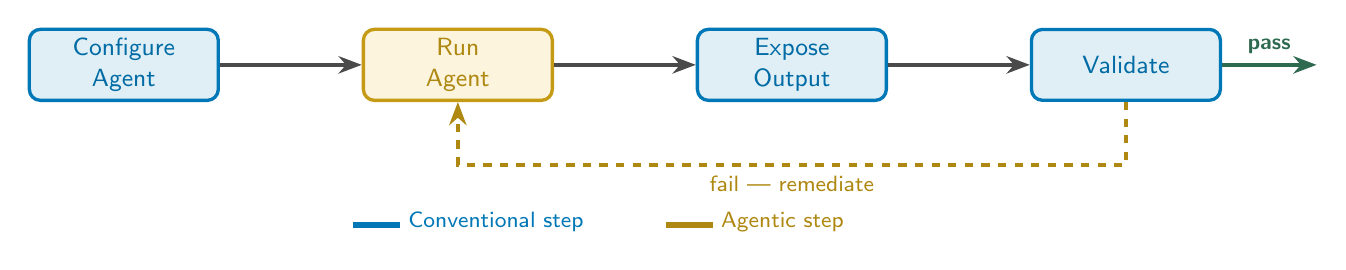
\begin{tikzpicture}[
    >=Stealth,
    font=\sffamily\small,
    text=txtgray,
    node distance=1.4cm and 1.8cm,
    convbox/.style={
        draw=convblue, fill=convblue!12, rounded corners=4pt,
        minimum height=0.9cm, minimum width=2.4cm, align=center,
        font=\sffamily\small, text=convblue!90!black,
        line width=1.2pt,
    },
    agentbox/.style={
        draw=agentamber!85!black, fill=agentamber!15, rounded corners=4pt,
        minimum height=0.9cm, minimum width=2.4cm, align=center,
        font=\sffamily\small, text=agentamber!75!black,
        line width=1.2pt,
    },
    arr/.style={->, very thick, color=txtgray},
    failarr/.style={->, very thick, color=failred, dashed},
]

% Nodes
\node[convbox] (prepare) {Configure\\Agent};
\node[agentbox, right=of prepare] (agent) {Run\\Agent};
\node[convbox, right=of agent] (expose) {Expose\\Output};
\node[convbox, right=of expose] (validate) {Validate};

% Main flow arrows
\draw[arr] (prepare) -- (agent);
\draw[arr] (agent) -- (expose);
\draw[arr] (expose) -- (validate);

% Pass arrow out
\draw[arr, passgreen] (validate.east) -- ++(1.2,0) node[above, midway, font=\sffamily\footnotesize\bfseries, passgreen] {pass};

% Retry loop
\draw[->, very thick, color=agentamber!75!black, dashed] (validate.south) -- ++(0,-0.8) -| node[below, near start, font=\sffamily\footnotesize, agentamber!75!black] {fail — remediate} (agent.south);

% Legend — centered between prepare and validate
\path (prepare.west) -- (validate.east) coordinate[midway] (diag center);
\node[convblue, font=\sffamily\footnotesize, anchor=east] at ([xshift=-0.4cm, yshift=-2.0cm]diag center)
    {\rule{0.6cm}{2pt}\ Conventional step};
\node[agentamber!75!black, font=\sffamily\footnotesize, anchor=west] at ([xshift=0.4cm, yshift=-2.0cm]diag center)
    {\rule{0.6cm}{2pt}\ Agentic step};

\end{tikzpicture}
\end{document}
